\chapter{Analyse et Conception} % Main chapter title

\label{Chapitre 2} % For referencing the chapter elsewhere, use \ref{Chapter1} 

\lhead{Chapitre 2. \emph{Analyse et Conception}} % This is for the header on each page - perhaps a shortened title

%----------------------------------------------------------------------------------------

\section{Le Backlog du Produit}
Le backlog du produit est la liste des fonctionnalités attendues d'un produit. Plus exactement, au-delà de cet aspect fonctionnel, il contient tous les éléments qui vont nécessiter du travail pour l'équipe. Les éléments y sont classés par priorité ce qui permet de définir l'ordre de réalisation.\\[0.5cm]
Le backlog est élaboré avant le lancement des sprints, dans la phase de préparation (ou sprint 0). Il est utilisé pour planifier la release, puis à chaque sprint, lors de la réunion de planification du sprint pour décider du sous-ensemble qui sera réalisé.\\[0.2cm]
C'est donc un outil essentiel pour la planification. Mais il est aussi, par sa nature, un maillon de la gestion des exigences, puisqu'on y collecte ce que doit faire le produit.\\[0.2cm]
A tout moment, le backlog est visible par tout le monde.
\begin{figure}[h]
\begin{tabular}{|p{7cm}|p{4cm}|p{4cm}|}
\hline
\textbf{Story} & \textbf{Priorité2 } & \textbf{Effort ou chargen} \\
\hline
En tant qu'utilisateur, je souhaite pouvoir voir les news dans une fil d'actualité,et de sélectionner un contenu pour le visualiser. & \begin{center}M\end{center} & \begin{center}22\end{center}\\
\hline
En tant qu'utilisateur, je souhaite pouvoir ajouter un contenu au favoris pour que je puisse le visualiser plus tard. & \begin{center}C\end{center} & \begin{center}11\end{center}\\
\hline
En tant qu'utilisateur, je souhaite pouvoir visiter les différentes contenu par catégories,et de les sélectionner selon mon besoin. & \begin{center}M\end{center} & \begin{center}60\end{center}\\
\hline
\end{tabular}
  \caption{Le Backlog du Produit}
  \label{fig:Backlog}
\end{figure}
\subsection{La méthode de priorisation}
Pour prioriser le besoin, on a utilisé la méthode  \textbf{MoSCow} ; elle est une technique visant à prioriser des besoins ou des exigences en matière d'assistance à maîtrise d'ouvrage et de développement logiciel. L'objectif est que le maître d'œuvre et le maître d'ouvrage s'accordent sur l'importance des tâches à réaliser par rapport aux délais prévus.\\[0.2cm]
Les lettres majuscules de l'acronyme MoSCoW signifient (en anglais):\\[0.2cm]
\begin{description}
\item[M] must have this, c'est-à-dire 'doit être fait' (vital).
\item[S] should have this if at all possible, c'est-à-dire devrait être fait dans la mesure du possible (essentiel).
\item[C] could have this if it does not affect anything else, pourrait être fait dans la mesure où cela n'a pas d'impact sur les autres tâches (confort).
\item[W] won't have this time but would like in the future, ne sera pas fait cette fois mais sera fait plus tard' (luxe, c'est votre zone d'optimisation budgétaire).
\end{description}






\chapter{Sprint 0 : Preparation et étude de projet}
\label{Chapitre 3} % For referencing the chapter elsewhere, use \ref{Chapter1} 

\lhead{Chapitre 3. \emph{Sprint 0 : Preparation et étude de projet}} % This is for the header on each page - perhaps a shortened title

%----------------------------------------------------------------------------------------

\section{Spécification}
\subsection{Le Backlog du Sprint}


\begin{figure}[H]
\begin{tabular}{|p{7cm}|p{4cm}|p{4cm}|}
\hline
\textbf{Story} & \textbf{Priorité2 } & \textbf{Effort ou chargen} \\
\hline
En tant qu'utilisateur, je souhaite pouvoir voir les news dans une fil d'actualité,et de sélectionner un contenu pour le visualiser. & \begin{center}M\end{center} & \begin{center}22\end{center}\\
\hline
En tant qu'utilisateur, je souhaite pouvoir ajouter un contenu au favoris pour que je puisse le visualiser plus tard. & \begin{center}C\end{center} & \begin{center}11\end{center}\\
\hline
\end{tabular}
  \caption{Le Backlog du Sprint 0}
  \label{fig:Backlog}
\end{figure}
\section{Conception}
\subsection{Diagramme de cas d’utilisation : services client}
Comme on peut voir dans le digramme \textbf{FIG.3.2} , on a trois acteurs : le client, l'administrateur, et le modèle de machine learning de classification.\\[0.2cm]
\begin{figure}[h]
	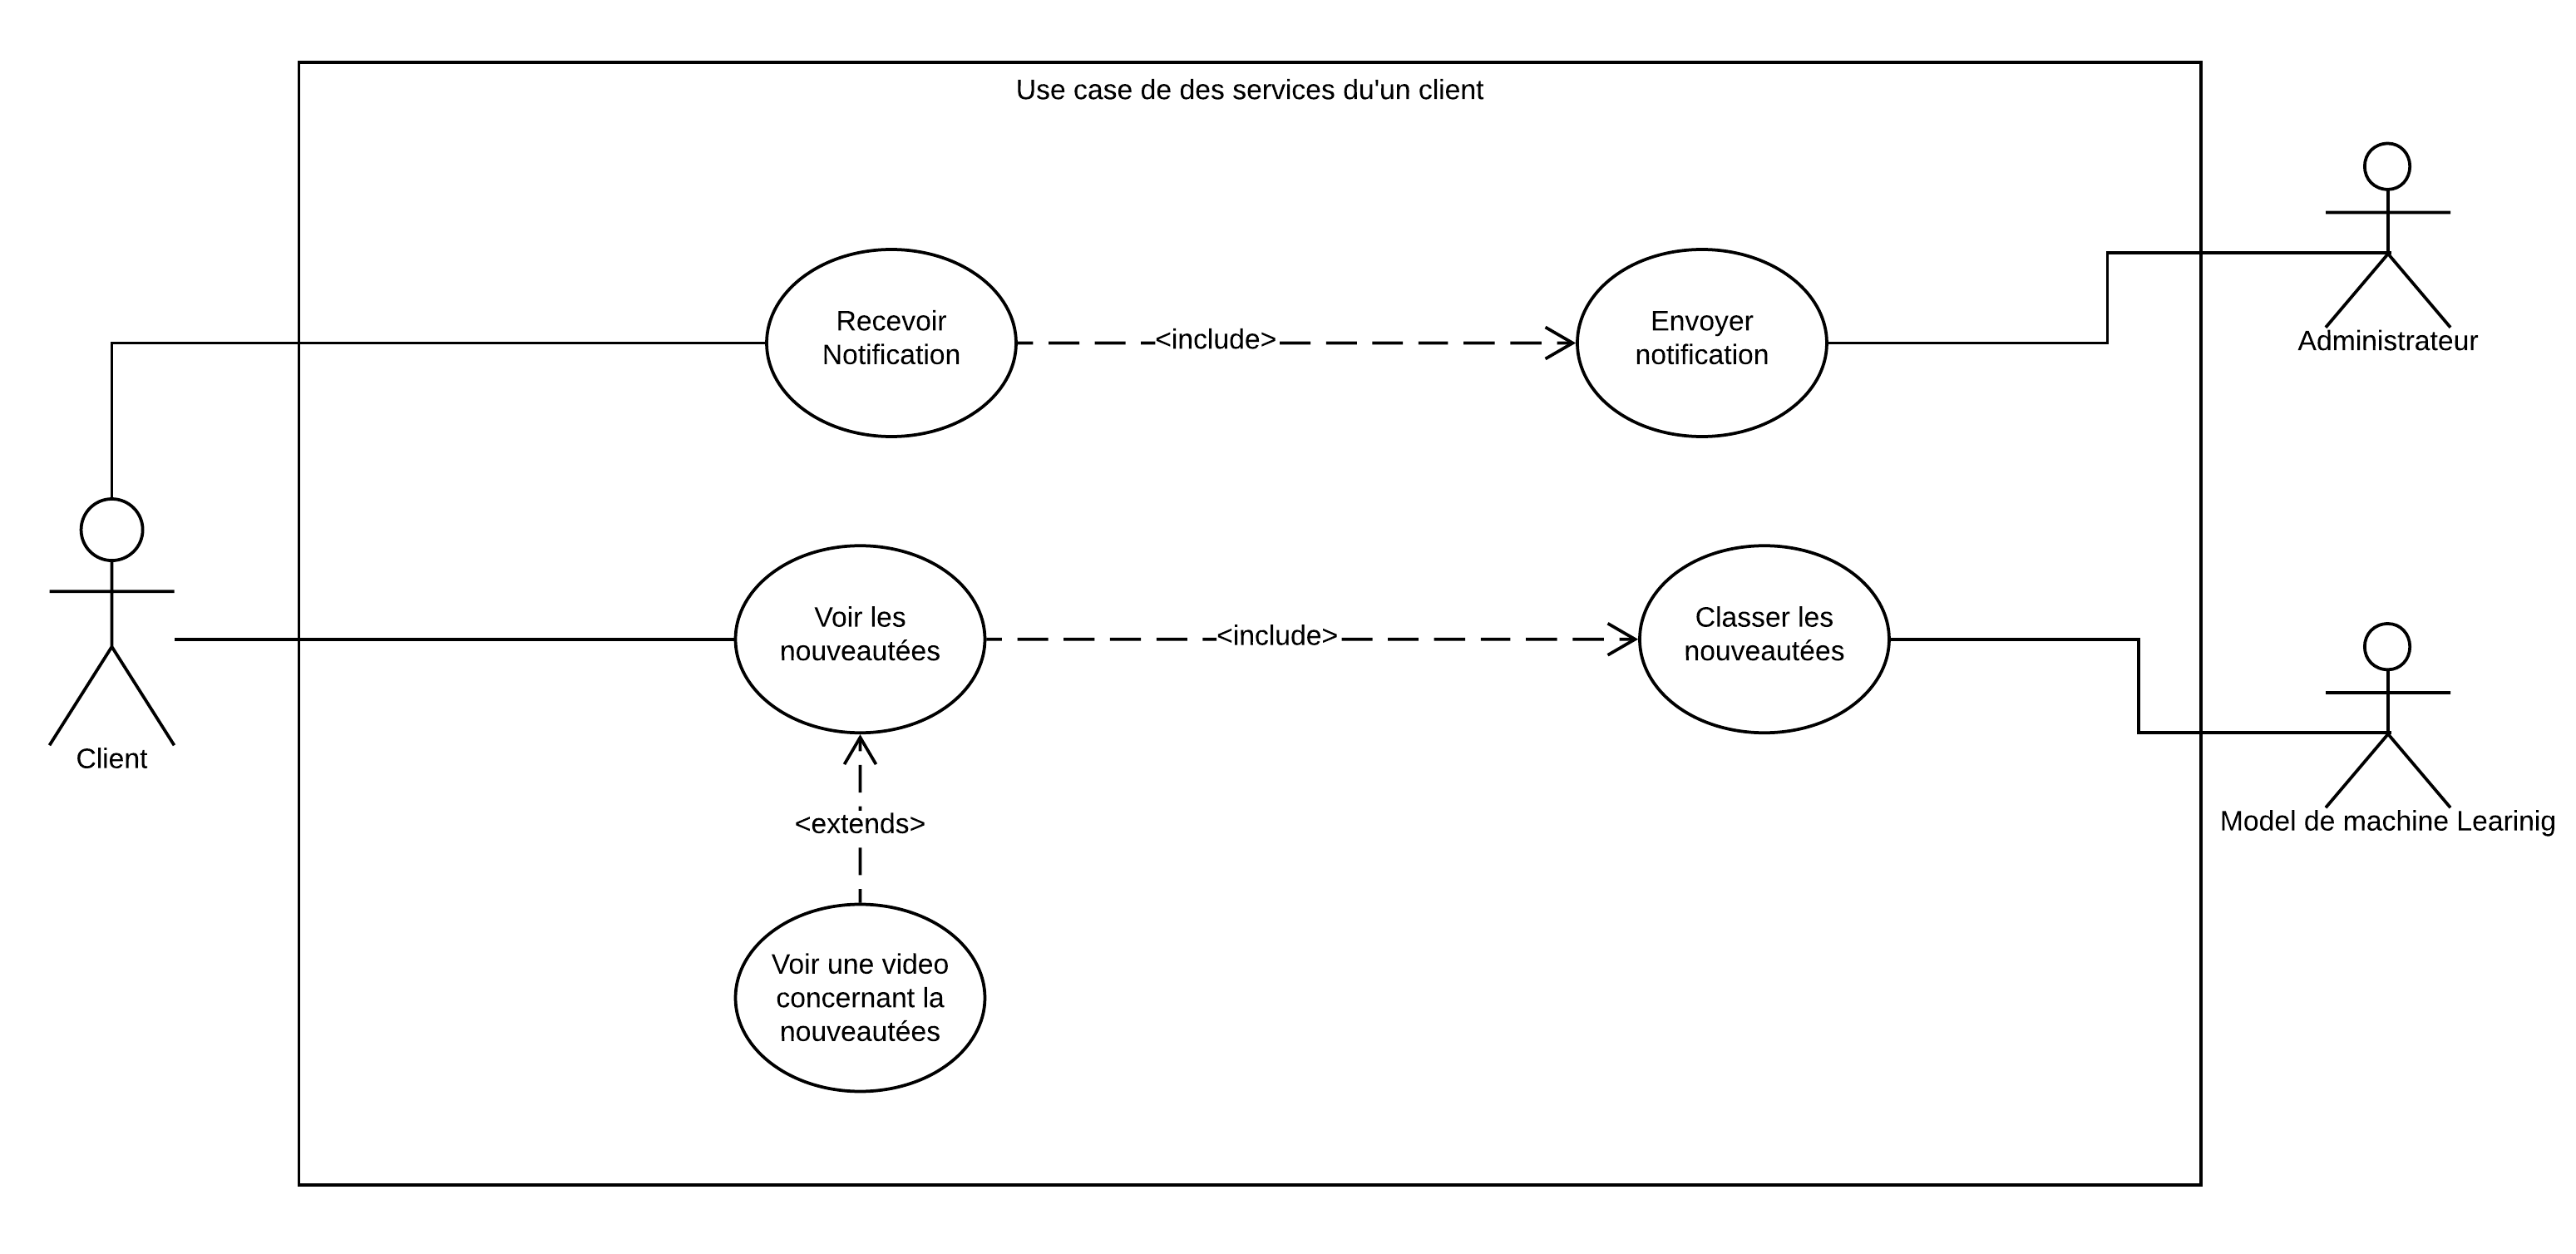
\includegraphics[scale=0.71]{Images/use_case_sanadtech.png}
	\caption{Diagramme de cas d'utilisation}
	\label{fig:cas-utilisation}
\end{figure}

Pour que le client puisse visualiser les nouveautés , il faut que ces dernières soient classifier selon leurs catégories par le modèle, après cette manipulation, le client pourra naviguer dans la page d'accueil et voir les nouveautés .\\[0.2cm]
Quand l'administrateur verra qu'une nouveauté est pertinente, il va lancer une notification, laquelle le client va recevoir, et pourra la visualiser en exclusivité.

\subsection{Diagramme de classes}
Comme on peut voir dans le digramme de la figure \textbf{FIG.3.3} , on a cinq classes : User, News, Catégorie; ApiAtacker et le modèle.\\[0.2cm]
\begin{figure}[H]
	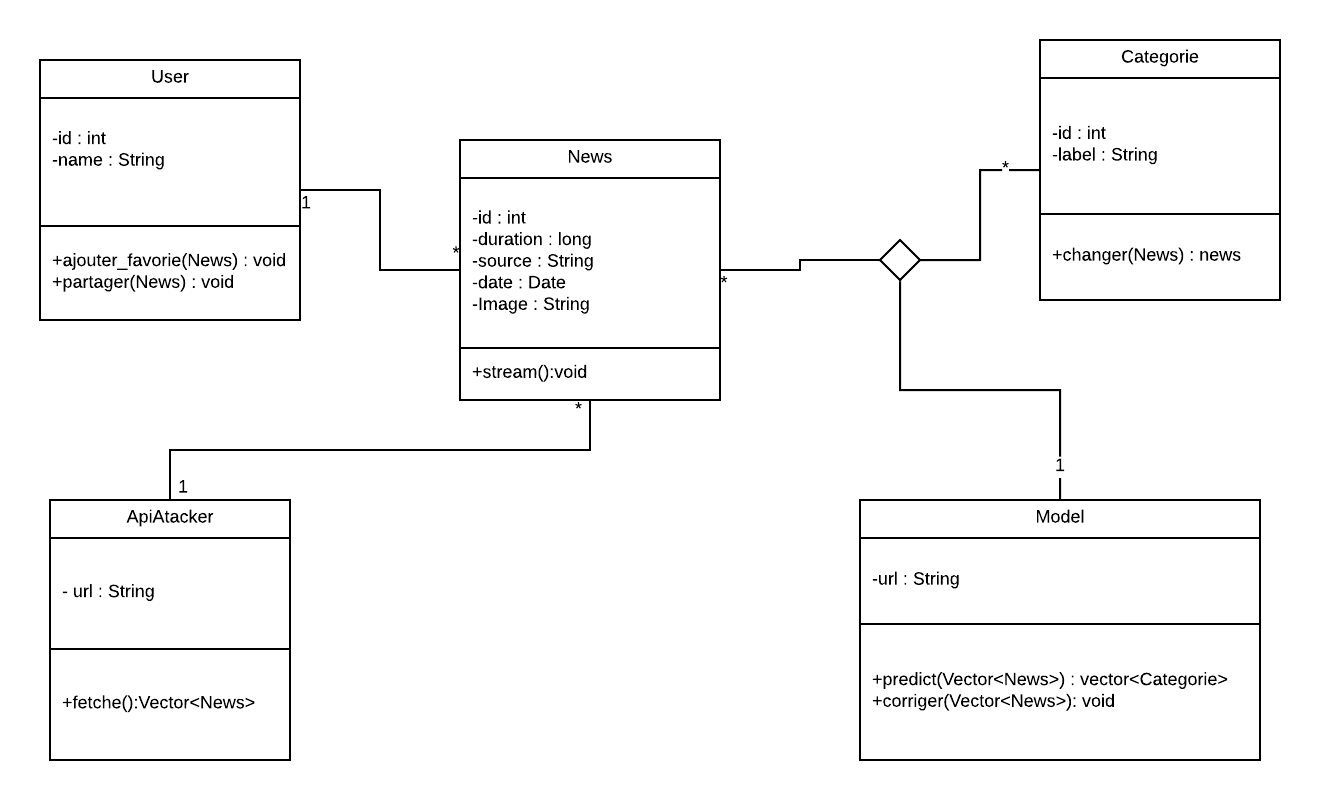
\includegraphics[scale=0.8]{Images/Class_diagram.png}
	\caption{Diagramme de classe}
	\label{fig:classe1}
\end{figure}

La classe \textbf{ApiAtacker},c'est la classe responsable de l'acquisition des données depuis les différentes sources qu'on a, tels que : youtube, hesspress ...\\[0.2cm]
La classe News représente une nouveauté dans notre système, et chaque nouveauté est lié par une et une seul catégorie.\\[0.2cm]
Ici, la classe Model joue le rôle du classificateur, elle est celle qui transforme une nouveauté non étiqueté en une qui est qui est  étiqueté.\\[0.2cm]
Par ces différentes méthode, la classe User représente un client dans notre système, il décrit toutes ses actions possible.

\subsection{Diagramme de séquence}
Comme vous pouvez constater dans le diagramme de la figure \textbf{FIG.3.4}, nous avons quatre ligne de vie dont le  Client, l'Application front-end, l'Application back-end,et le  Model tensorFlow.
\begin{figure}[H]
	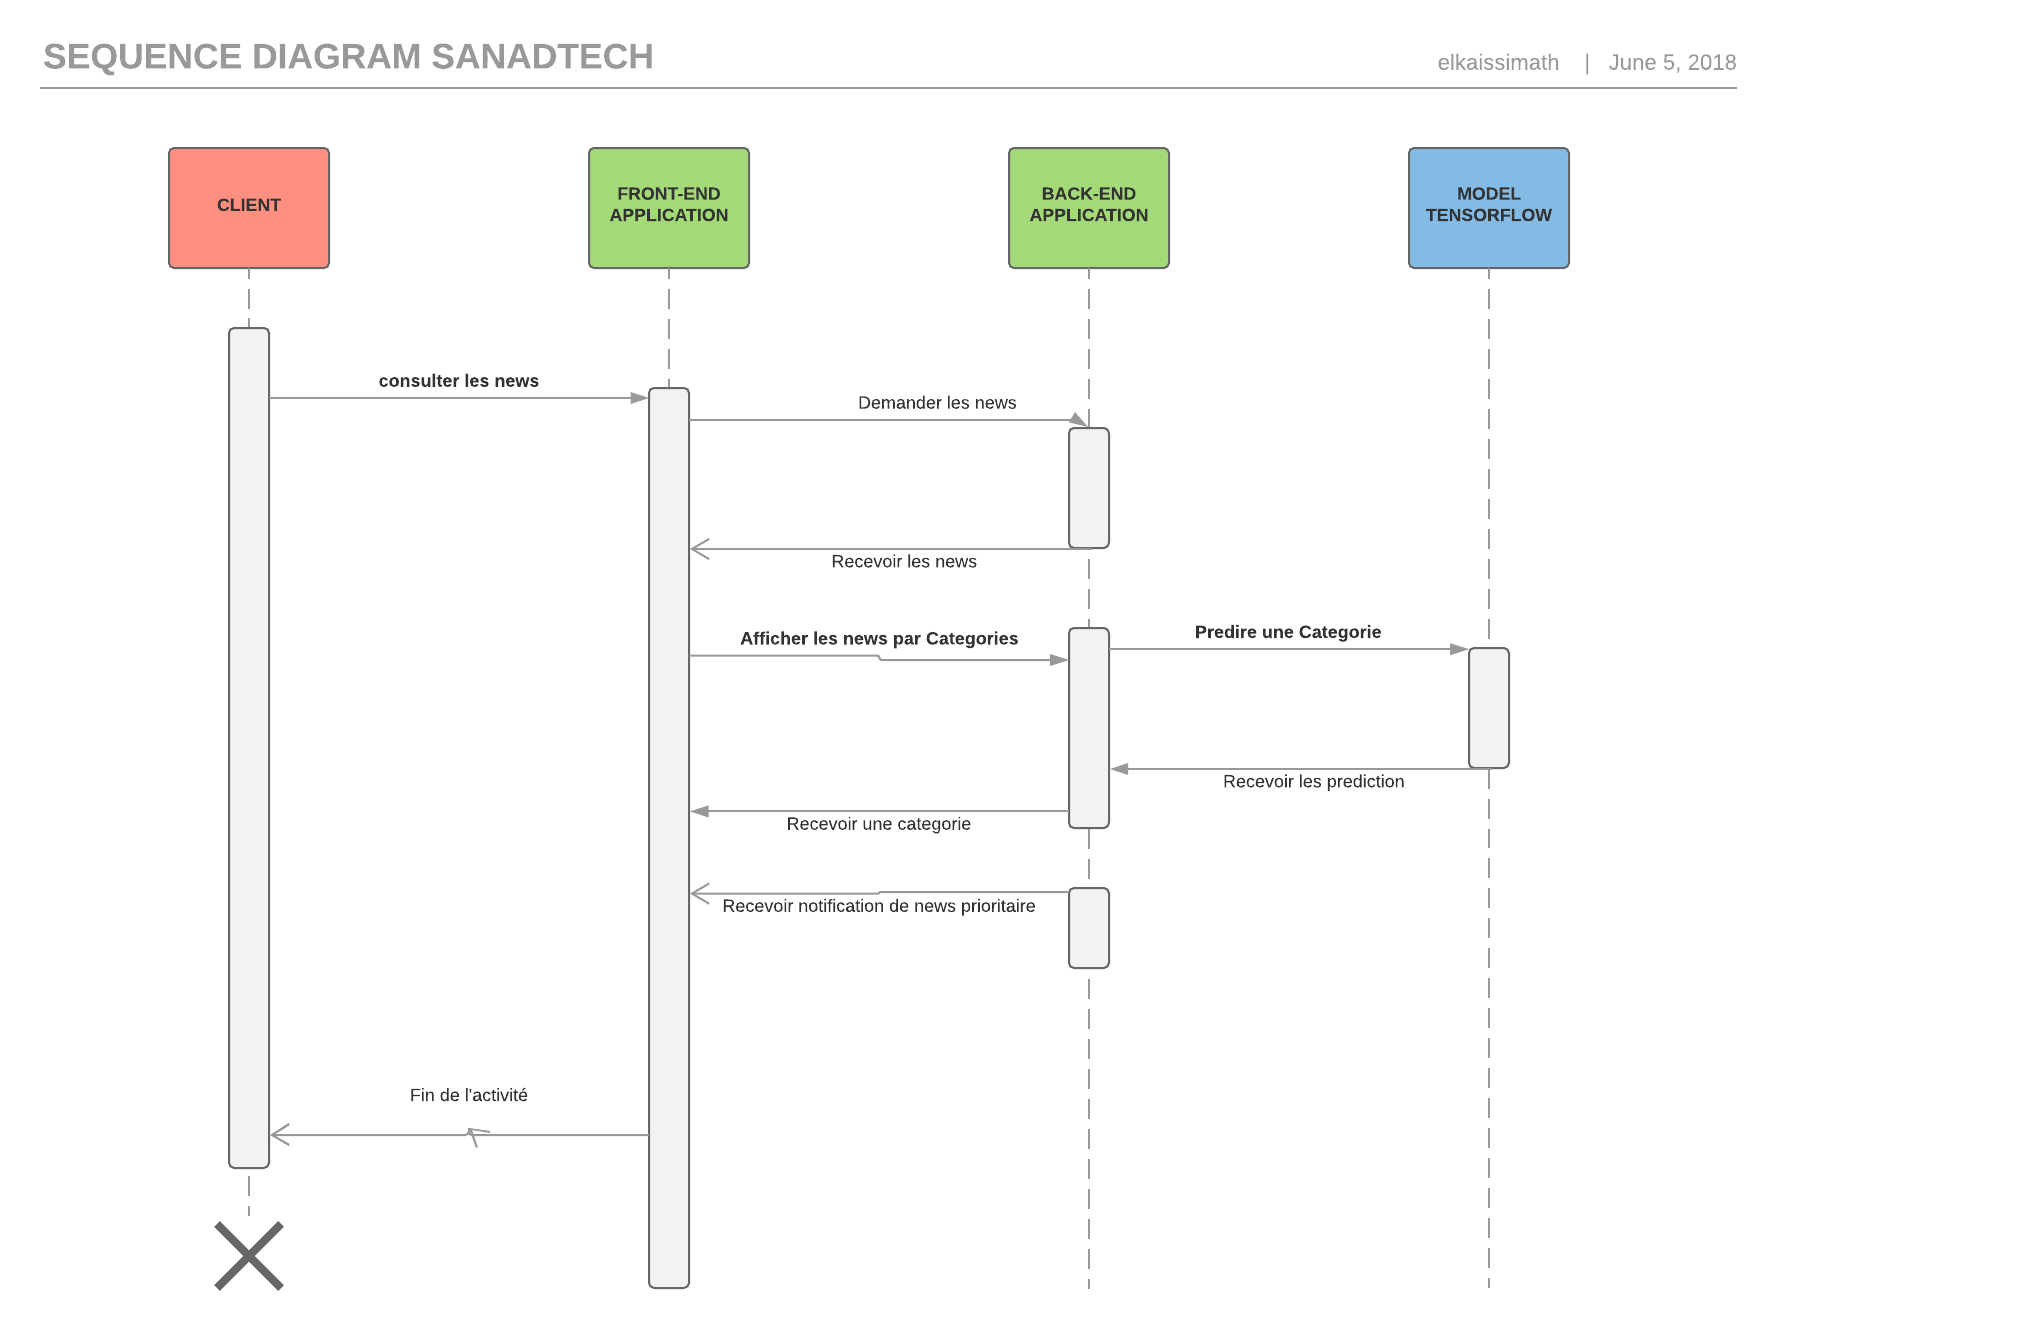
\includegraphics[scale=0.70]{Images/Sequence_Diagram_Sanadtech.png}
	\caption{Diagramme de séquence}
	\label{fig:sequence}
\end{figure}
L'activité de l'application au point de vue client commence, qu'on un utilisateur installe l'app dans son téléphone, il pourra ensuite recevoir les notifications des nouveautés les plus important.\\[0.2cm]
Quand un utilisateur consulte les nouveautés , le front-end envoi une requête au back-end, et ce dernier lui envoi tout les news par ordre de date.\\[0.2cm]
Si une news viens juste d'être intercepter par le back-end, elle envoi alors, une requête au modèle Tensorflow pour savoir de quelle catégorie cette news appartiens. Et puis après, le back-end l'enregistre avec ça nouvelle classe ou catégorie.\\[0.4cm]
Si une nouveauté est jugé comme importante, elle sera envoyer vers toutes les utilisateurs sous la forme d'une notifications, depuis le back-end.\\[0.2cm]

\subsection{Diagramme de déploiement}
Le diagramme de la figure \textbf{FIG.3.5} contient 4 nœuds principales, on site : front-end server, back-end server, database server , Model tensorflow server.
\begin{figure}[H]
	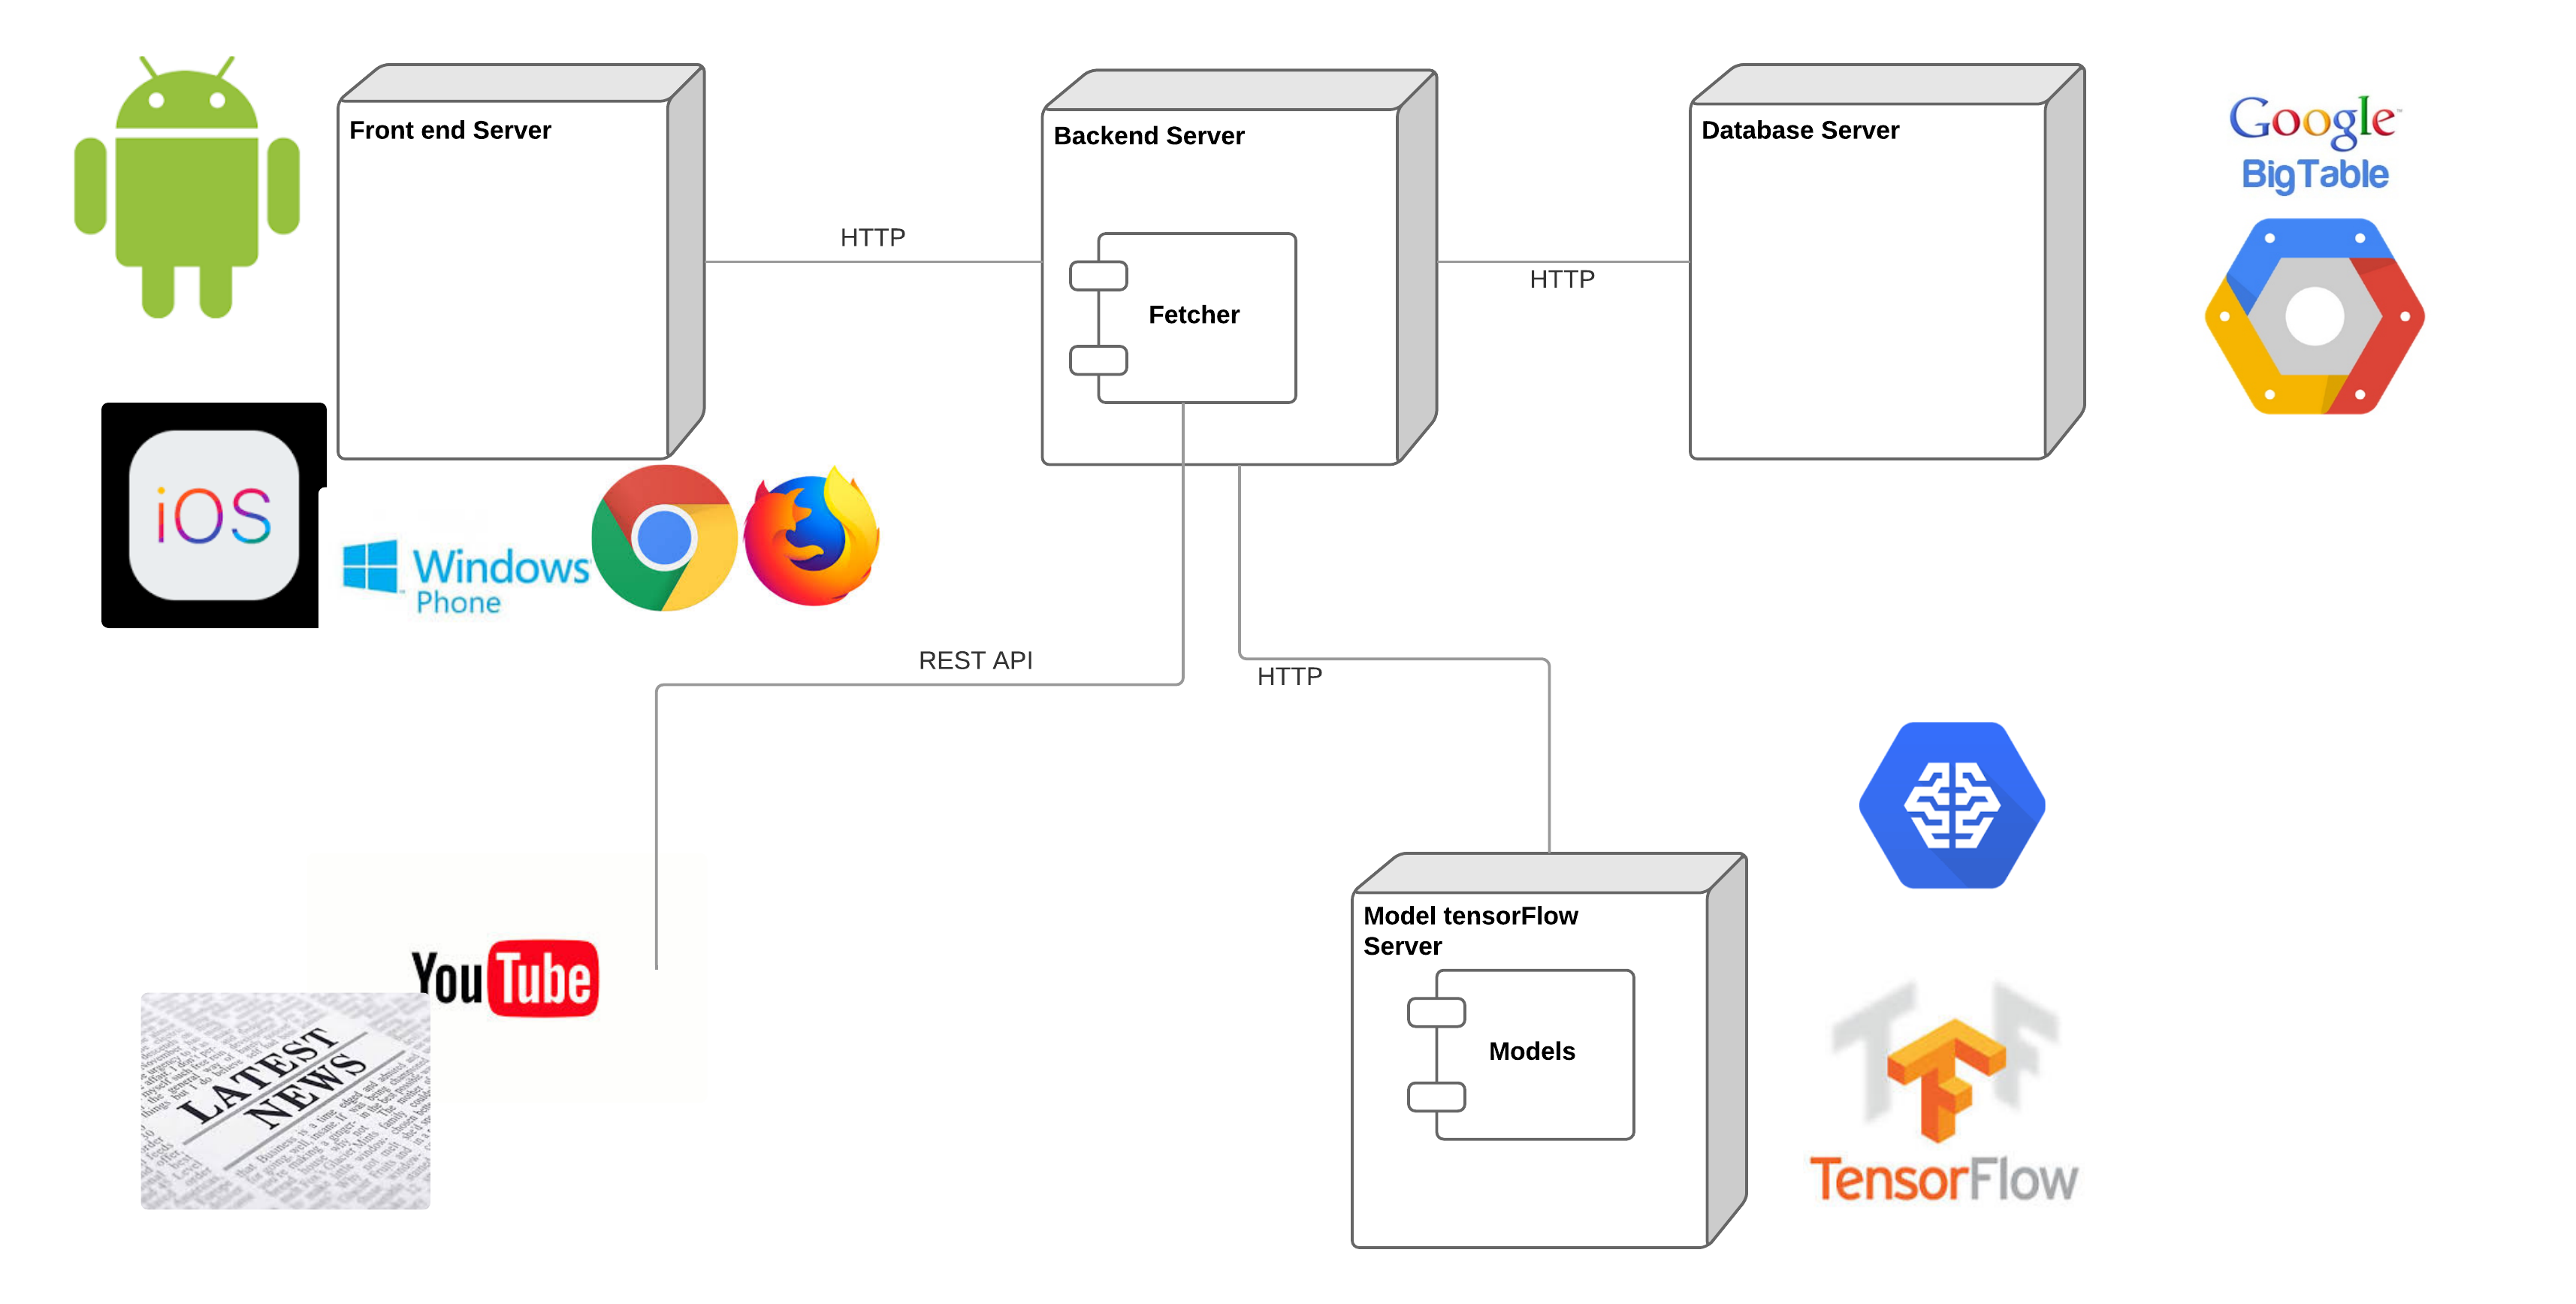
\includegraphics[width=\linewidth]{Images/Deployment_Diagram_Sanadtech.png}
	\caption{Diagramme de déploiement}
	\label{fig:deployment}
\end{figure}
Front-end server , c'est ou l'application finale est déployé, d'ici les utilisateurs peuvent la télécharger, depuis les différentes Stores, comme google play, apple store ...,ou la consulter dans le cas d'un navigateur.\\[0.2cm]
Back-end server, c'est ou le apiAtacker est situé , l'application envoi des requêtes vers ce nœud pour avoir les news.\\[0.2cm]
Database server, ici on stocke nos données , on utilise la base de donnée de google Big Table.\\[0.2cm]
Model Tensorflow Server, c'est ou notre model de prédiction est stocké , le modèle est écrit par tensorflow et déployer dans le service google ML-engine.



\section{NLP : Natural Language Processing}
Le modèle de classification qu'on va réaliser entre  dans la catégorie de la NLP, avant de le définir et l'expliquer, il faut d'abord rappeler qu'est ce que le machine learning et le deep learning.
\subsection{Machine learning}
L'apprentissage automatique (en anglais machine learning, littéralement « l'apprentissage machine ») ou apprentissage statistique, champ d'étude de l'intelligence artificielle, concerne la conception, l'analyse, le développement et l'implémentation de méthodes permettant à une machine (au sens large) d'évoluer par un processus systématique, et ainsi de remplir des tâches difficiles ou problématiques par des moyens algorithmiques plus classiques.\\[0.5cm]
L'analyse peut concerner des graphes, arbres, ou courbes (par exemple, la courbe d'évolution temporelle d'une mesure ; on parle alors de données continues, par opposition aux données discrètes associées à des attributs-valeurs classiques) au même titre que de simples nombres. Voir l'article Inférence bayésienne.\\[0.5cm]
Les algorithmes utilisés permettent, dans une certaine mesure, à un système piloté par ordinateur (un robot éventuellement), ou assisté par ordinateur, d'adapter ses analyses et ses comportements en réponse, en se fondant sur l'analyse de données empiriques provenant d'une base de données ou de capteurs.\\
La difficulté réside dans le fait que l'ensemble de tous les comportements possibles compte tenu de toutes les entrées possibles devient rapidement trop complexe à décrire (on parle d'explosion combinatoire). On confie donc à des programmes le soin d'ajuster un modèle pour simplifier cette complexité et de l'utiliser de manière opérationnelle. Idéalement, l'apprentissage visera à être non supervisé, c'est-à-dire que la nature des données d'entrainement n'est pas connue.\\[0.5cm]
Ces programmes, selon leur degré de perfectionnement, intègrent éventuellement des capacités de traitement probabiliste des données, d'analyse de données issues de capteurs, de reconnaissance (reconnaissance vocale, reconnaissance de forme, d'écriture…), de data-mining, d'informatique théorique…
\subsection{Deep Learning}
L'apprentissage profond1 (en anglais deep learning, deep structured learning, hierarchical learning) est un ensemble de méthodes d'apprentissage automatique tentant de modéliser avec un haut niveau d’abstraction des données grâce à des architectures articulées de différentes transformations non linéaires[réf. souhaitée]. Ces techniques ont permis des progrès importants et rapides dans les domaines de l'analyse du signal sonore ou visuel et notamment de la reconnaissance faciale, de la reconnaissance vocale, de la vision par ordinateur, du traitement automatisé du langage. Dans les années 2000, ces progrès ont suscité des investissements privés, universitaires et publics importants, notamment de la part des GAFA (Google, Apple, Facebook, Amazon).\\[0.5cm]
Les recherches dans ce domaine s’efforcent de construire de meilleures représentations du réel et de créer des modèles capables d’apprendre ces représentations à partir de données non labellisées à grande échelle. Certaines de ces représentations s’inspirent des dernières avancées en neuroscience. Il s'agit, grosso modo, d'interprétations du traitement de l’information et des modèles de communication du système nerveux, à l'image de la façon dont le système nerveux établit des connexions en fonction des messages reçus, de la réponse neuronale et du poids des connexions entre les neurones du cerveau.\\
Les différentes architectures de « deep learning » telles que les « deep neural networks », les « convolutional deep neural networks », et les « deep belief network » ont plusieurs champs d’application :
\begin{itemize}
\item la vision par ordinateur (reconnaissance de formes) ;
\item la reconnaissance automatique de la parole ;
\item le traitement automatique du langage naturel ;
\item la reconnaissance audio et la bio-informatique.
\end{itemize}
Dans ces deux derniers domaines, notamment, elles ont obtenu des résultats très prometteurs.
\subsection{NLP}
Le traitement automatique du langage naturel (abr. TALN), ou traitement automatique de la langue naturelle1, est un domaine multidisciplinaire impliquant la linguistique, l'informatique et l'intelligence artificielle. Il vise à créer des outils de traitement de la langue naturelle pour diverses applications. Il ne doit pas être confondu avec la linguistique informatique, qui vise à comprendre les langues au moyen d'outils informatiques.\\[0.5cm]
Le TALN est sorti des laboratoires de recherche pour être progressivement mis en œuvre dans des applications informatiques nécessitant l'intégration du langage humain à la machine2. Aussi le TALN est-il parfois appelé ingénierie linguistique3. En France, le traitement automatique de la langue naturelle a sa revue, ATALA, publiée par l’Association pour le traitement automatique des langues.




\section{Préparation des données}	
Dans un projet de machine learning, il est important de bien encadrer les données, parce que en sens large, il constitue l'enjeu majeur. Pour ce fait, on a suivi ces principaux étapes :
\subsection{Identification des sources de données}
Les données qu'on traite sont des données de type chaine de caractère qui comporte deux champs, le première champs et celui de la catégorie ou la classe, et le deuxième champs et celui de la description ou le titre de la vidéo.
\begin{figure}[H]
	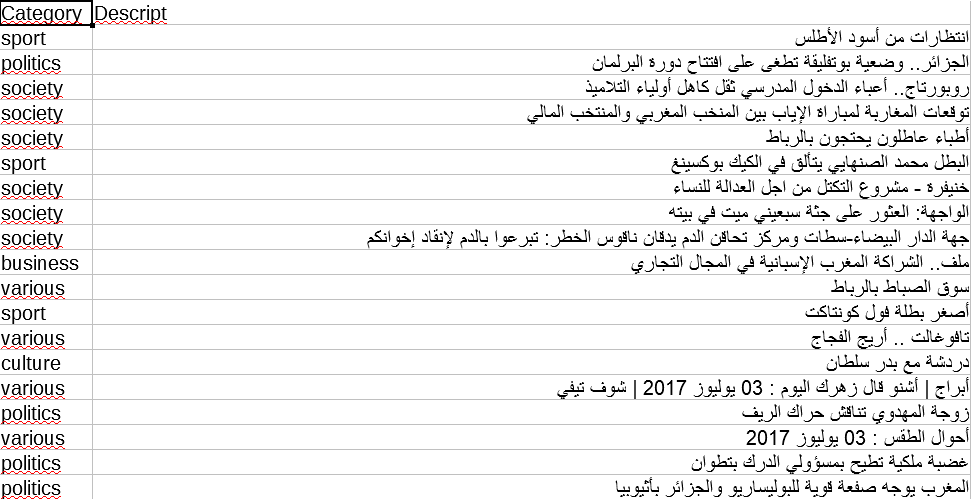
\includegraphics[width=\linewidth]{Images/donnees_contenu.png}
	\caption{Exemple de données}
	\label{fig:donnees}
\end{figure}	
Le format des données actuellement, avec lequelle on va faire l'entrainement et les testes, sont en format \textbf{CSV}, l'avantage de ce format c'est qu'il est facilement manipulable par le langage de programmation python même si la taille de données peut être grande.\\[0.2cm]
On récupère ses données là depuis plusieurs source, et après on extrait les données juger utiles pour les prédiction, dans ce cas les description des vidéo.
\subsection{Définition du lieu d'entreposage}
Les données transformé doivent etre stockés, pour le fait de ne pas les predire une deuxieme fois, on utilise dans notre projet la base données google, Big Table, il  est un système de gestion de base de données compressées, haute performance, et propriétaire, C'est une base de données orientée colonnes, dont se sont inspirés plusieurs projets libres, comme HBase, Cassandra ou Hypertable.\\
\begin{figure}[H]
	\begin{center}
	
\includegraphics[width=100mm,scale=0.5]{Images/google-cloud-bigtable.png}
	\end{center}
	\caption{google cloud big table}
	\label{fig:gglcloudbigtable}
\end{figure}	
 Google ne distribue pas sa base de données mais propose une utilisation publique de BigTable via sa plateforme d'application Google App Engine.
\subsection{Nettoyage des données}
Les données utilisées proviennent de diverses sources et processus et peuvent contenir des irrégularités ou des données corrompues compromettant la qualité de l'ensemble de données. Les problèmes typiques de qualité des données qui se posent sont les suivants:
\begin{description}
\item[Incomplet : ] Les données manquent d'attributs ou contiennent des valeurs manquantes.
\item[Noisy : ]les données contiennent des enregistrements erronés ou des valeurs aberrantes.
\item[Inconsistant : ]les données contiennent des enregistrements ou des divergences conflictuels.
\end{description}
Les données de qualité sont une condition préalable à la qualité des modèles prédictifs. Pour éviter les «déchets» et améliorer la qualité des données et donc la performance du modèle, nous avons trouvé qu'il est impératif de réaliser un écran d'intégrité des données afin de repérer rapidement les problèmes de données et de décider des étapes de traitement et de nettoyage correspondantes.
\subsection{Features generation}
C'est un processus consistant à prendre des données brutes non structurées et à définir des caractéristiques (c'est-à-dire des variables) pour une utilisation potentielle dans l'analyse statistique.\\
 Par exemple, dans le cas de l'exploration de texte \textit{(notre cas)}, on a  commencé avec un journal brut de milliers de descriptions \textit{(celles des vidéos)} et générer des fonctionnalités en supprimant des mots de faible valeur. des blocs de mots \textit{(n-grammes)} ou en appliquant d'autres règles.\\[0.5cm]
pour notre cas, on prend le corpus de données et on fait une relation symétrique entre les données de types chaine de caractère,et des entiers unique, qu'on le store par la suite dans un dictionnaire de données.
\subsection{Feature extration}
Une fois les fonctionnalités générées, il est souvent nécessaire de tester les transformations des entités d'origine et de sélectionner un sous-ensemble de ce groupe de caractéristiques potentielles originales et dérivées à utiliser dans notre modèle (extraction et sélection de caractéristiques).\\[0.2cm]
Tester des valeurs dérivées est une étape courante car les données peuvent contenir des informations importantes qui ont un modèle ou une relation non linéaire avec notre résultat, ainsi l'importance de l'élément de données peut seulement apparaître dans son état transformé (par exemple des dérivés d'ordre supérieur).\\[0.2cm]
 L'utilisation d'un trop grand nombre de caractéristiques peut entraîner une colinéarité multiple ou confondre des modèles statistiques, alors qu'extraire le nombre minimum de caractéristiques correspondant au but de votre analyse suit le principe de la parcimonie.\\[0.2cm]
\\On a divisé les données generées en deux parties, les données de d'entrainement qu'on lui a attribué 60\% des données du corpus, et les données de test qui formes un pourcentage de 40\%. 
\chapter{Sprint 1 : Réalisation d’un modèle de prédiction avec l’algorithme CNN}
\label{Chapitre 4} % For referencing the chapter elsewhere, use \ref{Chapter1} 

\lhead{Chapitre 4. \emph{Sprint 1 : Réalisation d’un modèle de prédiction avec l’algorithme CNN}} % This is for the header on each page - perhaps a shortened title

%----------------------------------------------------------------------------------------
\section{Spécification}
\subsection{Le Backlog du Sprint}
\begin{figure}[H]
\begin{tabular}{|p{7cm}|p{4cm}|p{4cm}|}
\hline
\textbf{Story} & \textbf{Priorité2 } & \textbf{Effort ou chargen} \\
\hline
En tant qu'utilisateur, je souhaite pouvoir visiter les différentes contenu par catégories,et de les sélectionner selon mon besoin. & \begin{center}M\end{center} & \begin{center}22\end{center}\\
\hline
\end{tabular}
  \caption{Le Backlog du Sprint 1}
  \label{fig:Backlog1}
\end{figure}


\section{Conception}

\subsection{Qu'est ce qu'un CNN/RNN ?}
\textbf{Réseau de neurones convolutifs}\\[0.5cm]
En apprentissage automatique, un réseau de neurones convolutifs ou réseau de neurones à convolution (en anglais CNN ou ConvNet pour Convolutional Neural Networks) est un type de réseau de neurones artificiels acycliques (feed-forward), dans lequel le motif de connexion entre les neurones est inspiré par le cortex visuel des animaux. Les neurones de cette région du cerveau sont arrangés de sorte qu'ils correspondent à des régions qui se chevauchent lors du pavage du champ visuelle.\\[0.2cm]
 Leur fonctionnement est inspiré par les processus biologiques, ils consistent en un empilage multicouche de perceptrons, dont le but est de pré-traiter de petites quantités d'informations. Les réseaux neuronaux convolutifs ont de larges applications dans la reconnaissance d'image et vidéo, les systèmes de recommandation et le traitement du langage naturel.\\[1cm]

 \textbf{Réseau de neurones récurrents}\\[0.5cm]
 
 Un réseau de neurones récurrents est un réseau de neurones artificiels présentant des connexions récurrentes. Un réseau de neurones récurrents est constitué d'unités (neurones) inter-connectés interagissant non-linéairement et pour lequel il existe au moins un cycle dans la structure. Les unités sont reliées par des arcs (synapses) qui possèdent un poids. La sortie d'un neurone est une combinaison non linéaire de ses entrées.\\[0.2cm]
Les réseaux de neurones récurrents sont adaptés pour des données d'entrée de taille variable. Ils conviennent en particulier pour l'analyse de séries temporelles. Ils sont utilisés en reconnaissance automatique de la parole ou de l'écriture manuscrite - plus en général en reconnaissance de formes - ou encore en traduction automatique. « Dépliés », ils sont comparables à des réseaux de neurones classiques avec des contraintes d'égalité entre les poids du réseau (voir schéma ci-dessous).

\begin{figure}[H]
	\begin{center}
	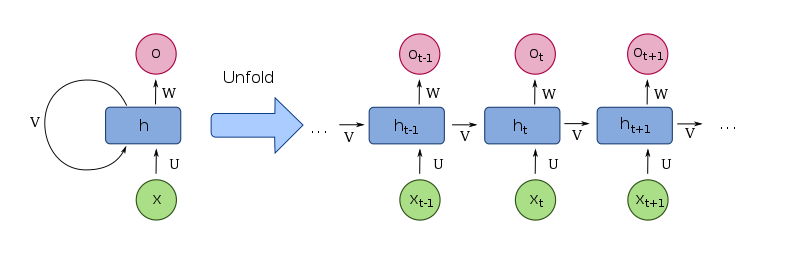
\includegraphics[width=100mm,scale=0.5]{Images/rnn.png}
	\end{center}
	\caption{Schéma d'un réseau de neurones récurrents à une unité reliant l'entrée et la sortie du réseau. A droite la version « dépliée » de la structure.}
	\label{fig:rnn}
\end{figure}


\subsection{L'architecture de notre réseaux neuronal}
Le réseaux neuronal qu'on a adopté est comme suite : 

\begin{figure}[H]
	\begin{center}
	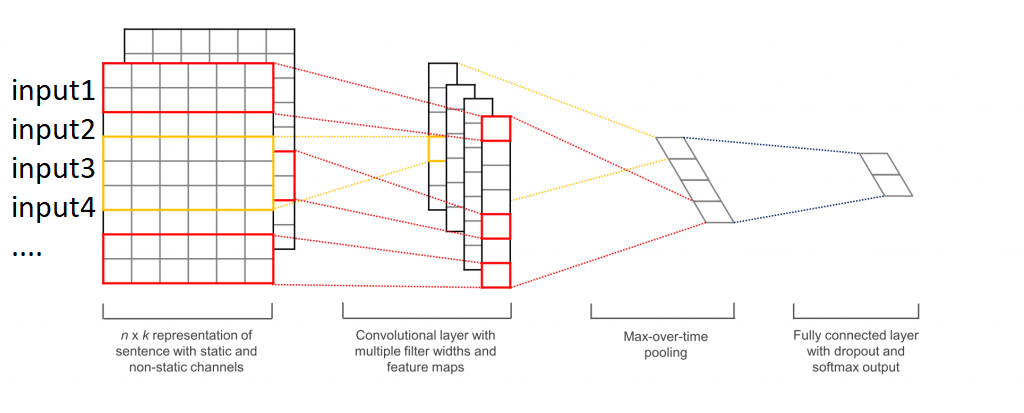
\includegraphics[width=\linewidth]{Images/cnn.png}
	\end{center}
	\caption{La structure du reseaux neuronal ,réaliser par cnn.}
	\label{fig:cnn1}
\end{figure}

Les premières couches incorpore des mots dans des vecteurs de basse dimension. La couche suivante effectue des convolutions sur les vecteurs de mots incorporés, en utilisant des tailles de filtres multiples.\\[0.2cm]

\begin{figure}[H]
	\begin{center}
	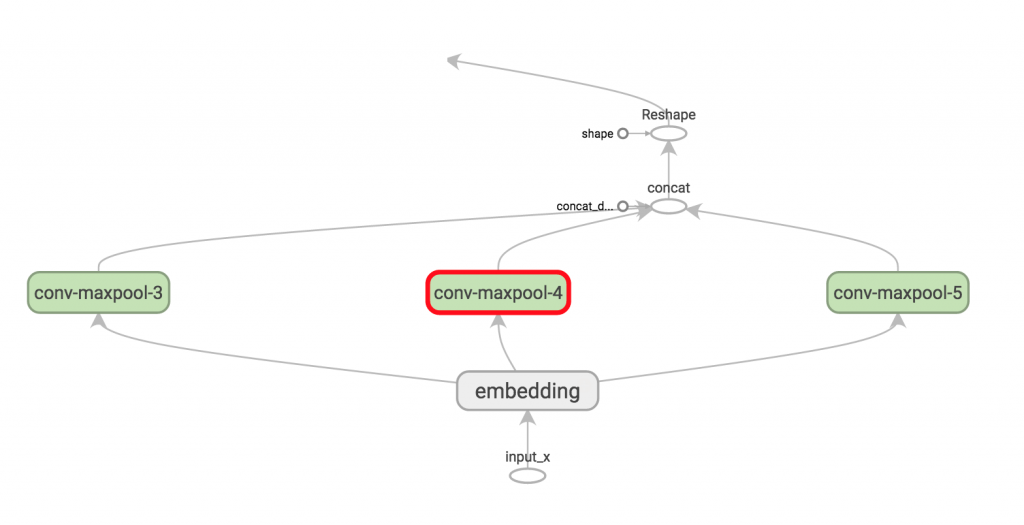
\includegraphics[width=\linewidth]{Images/cnn1.png}
	\end{center}
	\caption{La structure du réseaux neuronal, structure des couches de convolutions.}
	\label{fig:cnn1}
\end{figure}
 Par exemple, glisser sur 3, 4 ou 5 mots à la fois. Ensuite, nous max-poolons le résultat de la couche convolutionnelle dans un long vecteur de caractéristiques,et on ajoute une régularisation de décrochage, et en fin on  classe le résultat en utilisant une couche softmax.\\[0.5cm]
 
Puisque on ne peut pas traiter les chaînes de caractères dans un réseaux neuronal, on doit transformer ces données là, en des données numérique, c’est pour cela, j’ai utilisé une transformation classique « Embeding» qui mappe chaque mot qui existe dans mon dictionnaire de mot ,en des numéro significatif.\\[0.2cm]
Pour bien comprendre le déroulement ,et le processus de fonctionnement de ce réseaux neuronal , voici une figure descriptive :

\begin{figure}[H]
	\begin{center}
	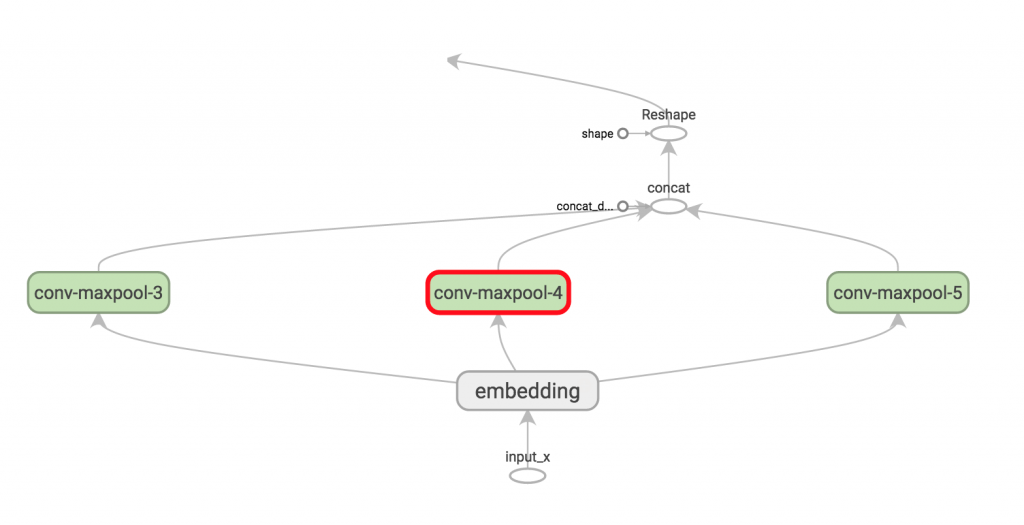
\includegraphics[width=\linewidth]{Images/cnn1.png}
	\end{center}
	\caption{Architecture des couches du réseaux neuronal.}
	\label{fig:cnn2}
\end{figure}

Ici, \textbf{W} est notre matrice de filtre et h est le résultat de l'application de la non-linéarité à la sortie de la convolution. Chaque filtre glisse sur l'ensemble de l'incorporation, mais varie en nombre de mots. Le remplissage \textit{VALIDE} signifie que nous glissons le filtre sur notre phrase sans capitonner les bords, en effectuant une convolution étroite qui nous donne une sortie de forme $ [1, sequenceLengthFilterSize+1, 1, 1] $.\\[0.2cm]
 L'exécution de \textbf{max-pooling} sur la sortie d'une taille de filtre spécifique nous laisse avec un tenseur de forme $ [batchSize, 1, 1, numFilters] $. C'est essentiellement un vecteur de caractéristiques, où la dernière dimension correspond à nos caractéristiques.\\[0.2cm]
Une fois que nous avons tous les tenseurs de sortie regroupés de chaque taille de filtre, nous les combinons en un long vecteur de forme de forme $ [tailleBatch, numFiltersTotal] $. \\[0.2cm]
L'utilisation de -1 dans tf.reshape indique à TensorFlow d'aplatir la cote lorsque cela est possible.\\[0.2cm]

Pour régulariser notre CNN, j’ai utilisé une couche \textbf{Dropout} ,l'idée derrière  est simple. Une couche de décrochement stochastique \textbf{désactive} une fraction de ses neurones. Cela empêche les neurones de co-adapter, et les oblige à apprendre des fonctionnalités utiles individuellement.\\[0.2cm]
 La fraction de neurones que nous gardons activée est définie sur notre réseau. Nous avons réglé ceci à quelque chose comme \textit{0.5} pendant l'entraînement, et à \textit{1} (désactiver la couche) pendant l'évaluation.\\[0.2cm]
 
 En utilisant le vecteur de caractéristiques de \textbf{max-pooling} (avec \textbf{dropout} appliqué), nous pouvons générer des prédictions en faisant une multiplication matricielle et en choisissant la classe ayant le score le plus élevé. Nous pourrions également appliquer une fonction \textbf{softmax} pour convertir les scores bruts en probabilités normalisées, mais cela ne changerait pas nos prédictions finales.\\[0.2cm]
 
 En utilisant nos \textit{scores}, nous pouvons définir la fonction de perte. La perte est une mesure de l'erreur que notre réseau fait, et notre objectif est de le minimiser. La fonction de perte standard pour la catégorisation pose des problèmes de perte d'\textit{entropie} croisée.\\[0.5cm]
Enfin le graphe final résultant ressemble à ça :
\begin{figure}[H]
	\begin{center}
	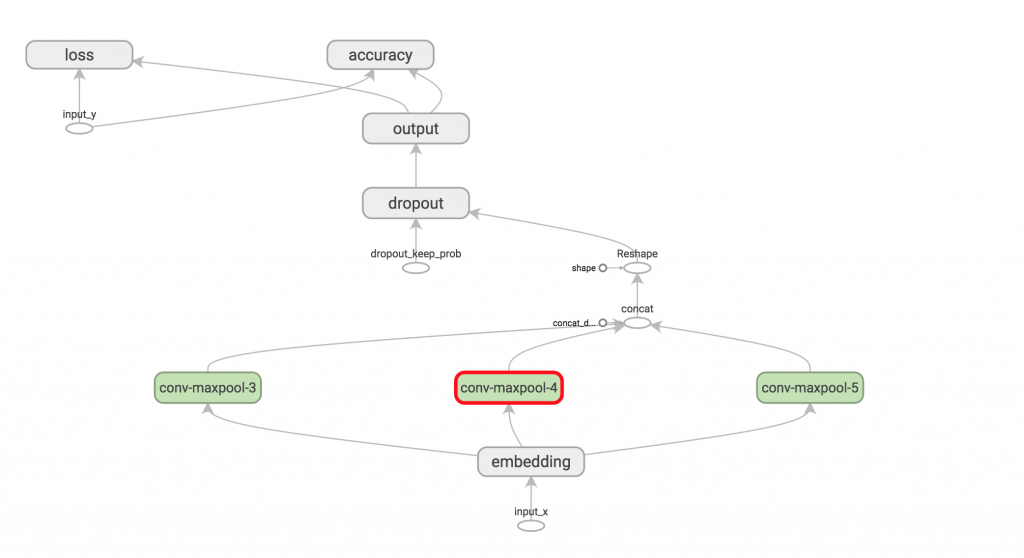
\includegraphics[width=\linewidth]{Images/cnn3.png}
	\end{center}
	\caption{Graphe qui représente les étapes du traitement du modèle.}
	\label{fig:rnn}
\end{figure}


 L’état des pertes sur les variables de décision :

\begin{figure}[H]
	\begin{center}
	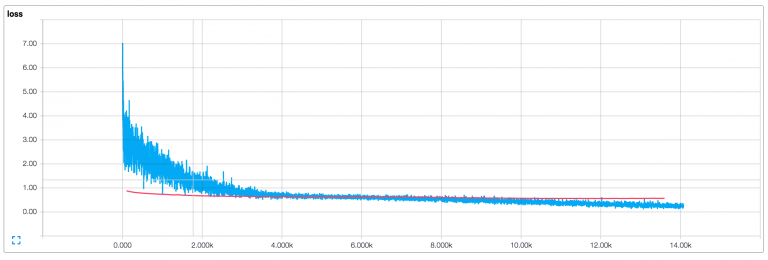
\includegraphics[width=\linewidth]{Images/cnn4.png}
	\end{center}
	\caption{Graphe qui représente les données perdues, du reseaux CNN/RNN.}
	\label{fig:rnn}
\end{figure}
 l'état des précision qui est égale à 0,76:
\begin{figure}[H]
	\begin{center}
	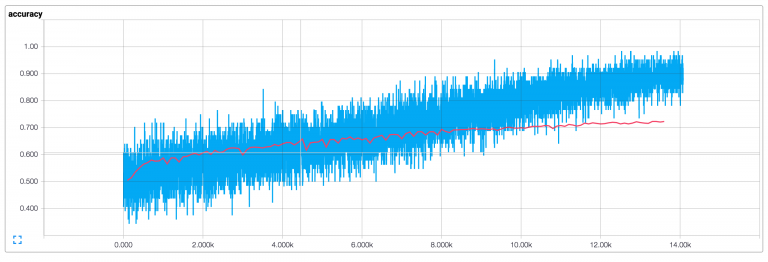
\includegraphics[width=\linewidth]{Images/cnn5.png}
	\end{center}
	\caption{Graphe qui représente la précision, du reseaux CNN/RNN}
	\label{fig:rnn}
\end{figure}




\chapter{Sprint 2 : Réalisation d’un modèle de prédiction avec l’algorithme SVM}
\label{Chapitre 5} % For referencing the chapter elsewhere, use \ref{Chapter1} 

\lhead{Chapitre 5. \emph{Sprint 2 : Réalisation d’un modèle de prédiction avec l’algorithme SVM}} % This is for the header on each page - perhaps a shortened title

%----------------------------------------------------------------------------------------
\section{Spécification}
\subsection{Le Backlog du Sprint}
\begin{figure}[H]
\begin{tabular}{|p{7cm}|p{4cm}|p{4cm}|}
\hline
\textbf{Story} & \textbf{Priorité2 } & \textbf{Effort ou chargen} \\
\hline
En tant qu'utilisateur, je souhaite pouvoir visiter les différentes contenu par catégories,et de les sélectionner selon mon besoin. & \begin{center}M\end{center} & \begin{center}22\end{center}\\
\hline
\end{tabular}
  \caption{Le Backlog du Sprint 2}
  \label{fig:Backlog2}
\end{figure}
\section{Conception}
\subsection{Qu'est ce que le SVM ?}
Les machines à vecteurs de support ou séparateurs à vaste marge (en anglais support vector machine, SVM) sont un ensemble de techniques d'apprentissage supervisé destinées à résoudre des problèmes de discrimination 1 et de régression. Les SVM sont une généralisation des classifieurs linéaires.\\[0.5cm]
Les séparateurs à vaste marge ont été développés dans les années 1990 à partir des considérations théoriques de Vladimir Vapnik sur le développement d'une théorie statistique de l'apprentissage : la théorie de Vapnik-Chervonenkis. Ils ont rapidement été adoptés pour leur capacité à travailler avec des données de grandes dimensions, le faible nombre d'\textbf{hyperparamètres}, leurs garanties théoriques, et leurs bons résultats en pratique.\\[0.5cm]
\begin{figure}[H]
	\begin{center}
	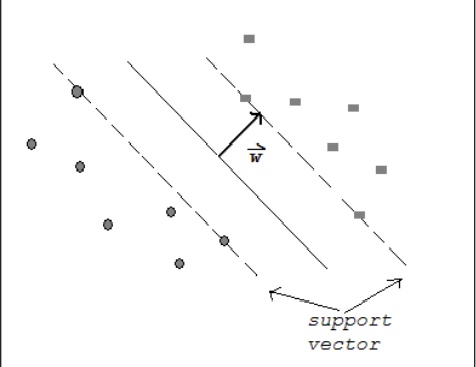
\includegraphics[scale=0.5]{Images/ex_svm.png}
	\end{center}
	\caption{Exemple d'un hyperplan pattern de SVM}
	\label{fig:svm0}
\end{figure}
Les SVM ont été appliqués à de très nombreux domaines (bio-informatique, recherche d'information, vision par ordinateur, finance…). Selon les données, la performance des machines à vecteurs de support est de même ordre, ou même supérieure, à celle d'un réseau de neurones ou d'un modèle de mélanges gaussiens.\\[1cm]
Les machines à vecteurs de support sont basées sur le principe de la structure de minimisation de risque, dans la théorie de l'apprentissage aléatoire.L'idée de la structure de minimisation de risque est de trouver une hypothèse \textbf{\textit{h}} avec laquelle on peut garantir, d'avoir le plus petit cout d'erreur. \\La vrai erreur de \textbf{\textit{h}}, c'est la probabilité que \textbf{\textit{h}} va faire une erreur en une données non traiter,et choisit aléatoirement. Un extremum haut, peut être utiliser, pour connecter, la vrai erreur de \textbf{\textit{h}}, avec l'erreur de \textbf{\textit{h}} et avec les données de  l'entrainement, est une complexité \textbf{\textit{H}} (mesurer par VC-Dimension), l'hypothèse \textbf{\textit{h}}, laquelle approximativement, minimise l'extremum pour la vrai valeur de \textbf{\textit{h}} en controllant the VC-Dimension de \textbf{\textit{H}}. \\[0.2cm]
Les SVMs, sont des apprentis universelles. Dans leur frome de base, ils apprennent par  des fonctions seuil linéaire. Sauf que par une utilisation des fonction de kernel à la place des variables unitaires, ils peuvent être utiliser pour un apprentissage polynomiale, et produire de classificateurs polynomiale.\\[0.2cm]
Autre chose qui est magnifique chez le SVM,c'est que son pouvoir d'apprentissage est indépendante du dimension de l'espace du features, il mesure la complexité de l'hypothèse basé sur la marge qui sépare les données, non le nombre des features. Ceci signifie qu'on peut généraliser, si notre données est séparable avec une grande fonction de marge, même en présence de plusieurs features.\\[0.2cm]
La marge suggère aussi d'avoir une heuristique pour sélectionner des valeurs exactes de traitement pour l'apprenti (comme le kernel avec le réseaux RBF). le meilleurs paramétrage, est celui qui produit l'hypothèse avec le plus petit VC-Dimension. Ceci permet d'automatiser les paramètres sans une perte de la cross-valisation.
\subsection{implémentation et optimisation}


On utilise le SVM dans les problèmes de classification binaires, or dans notre cas on 7 catégories.
Pour ce fait , il y a deux approche pour remédier à cette problématique :\\[1cm]
\textbf{Un contre tout le monde}\\[1cm]
Dans cette approche, on construit \textit{k} classificateurs  binaires séparés
pour la classification k-class. Le classificateur binaire m-th est formé en utilisant les données de
la m-ième classe comme exemples positifs et les classes k-1 restantes comme négatives
exemples.\\[0.2cm]
Pendant le test, l'étiquette de classe est déterminée par le classificateur binaire
donne la valeur de sortie maximale. Un problème majeur de l'approche un versus repos est
l'ensemble d'entraînement déséquilibré. Supposons que toutes les classes ont une taille égale d'entraînement exemples, le ratio d'exemples positifs à négatifs dans chaque classificateur est
$ 1/(1-k) $. Dans ce cas, la symétrie du problème original est perdue. \\[1cm]
\textbf{Un contre Un}\\[1cm]
Une autre approche classique pour la classification multi-classe est le Un contre Un (1V1)
ou une décomposition par paires . Il évalue tous les classificateurs par paires possibles et ainsi
induit $ k *(k - 1) / 2 $ classificateurs binaires individuels. Appliquer chaque classificateur à un test
exemple donnerait un vote à la classe gagnante. \\[0.5cm]
Un exemple de test est libellé pour la classe avec le plus de votes. La taille des classificateurs créés par le un contre un approche est beaucoup plus grande que celle de l'approche un versus repos.\\[0.5cm] Cependant, la taille de QP dans chaque classificateur est plus petit, ce qui permet de s'entraîner rapidement. De plus, par rapport à l'approche un contre le repos, la méthode un-contre-un est plus
symétrique. Platt et al. a amélioré l'approche un-contre-un et proposé
une méthode appelée SVM Directed Acyclic Graph SVM (DAGSVM) qui forme un arbre
structure pour faciliter la phase de test. En conséquence, il ne faut que k - 1 individu
évaluations pour décider de l'étiquette d'un exemple de test.\\[1.5cm]

J'ai essayé les deux méthode, avec l'utilisation du kernel gaussiens pour les deux cas, et aussi en variant la valeur de la variables gamma, et j'ai conclue après les testes sur les deux modèles que le (Un contre Un) et mieux adapté pour notre cas.\\
Puisque qu'on a 7 catégorie, le nombre de modèles utiliser est 21, chaque modèle sert à classifier la description entre deux classes, et c'est sur qu'il va y avoir un résultat .
\begin{figure}[H]
	\begin{center}
	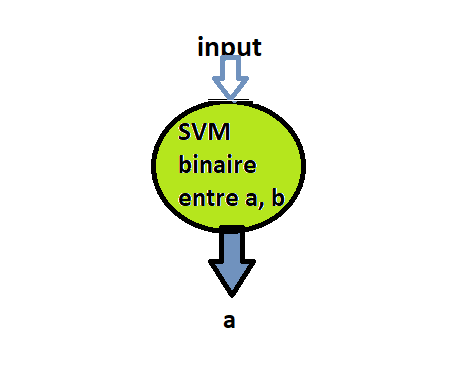
\includegraphics[scale=0.7]{Images/svm_binaire.png}
	\end{center}
	\caption{Représentation d'un modèle binaire SVM}
	\label{fig:svm0}
\end{figure}
L'algorithme utilisé consiste à faire les prédiction dans chaque modèle qu'on a , et puis après en regroupe le résultat finale dans un vecteur, qui contient lui aussi les valeurs d'apparition d'une classe dans une prédiction, on le résultat final, est la classe qui a apparu le plus, dans le vecteur .
\begin{figure}[H]
	\begin{center}
	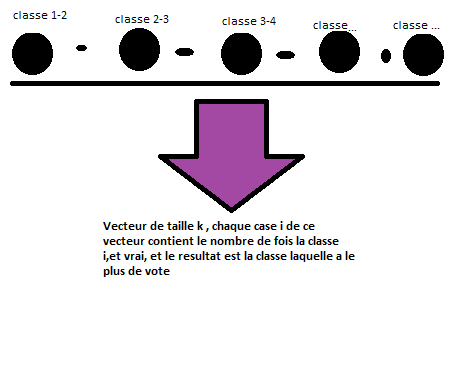
\includegraphics[scale=0.7]{Images/svm_rep.png}
	\end{center}
	\caption{Représentation globale du modèle}
	\label{fig:svm0}
\end{figure}



 L’état des pertes sur les variables de décision :

\begin{figure}[H]
	\begin{center}
	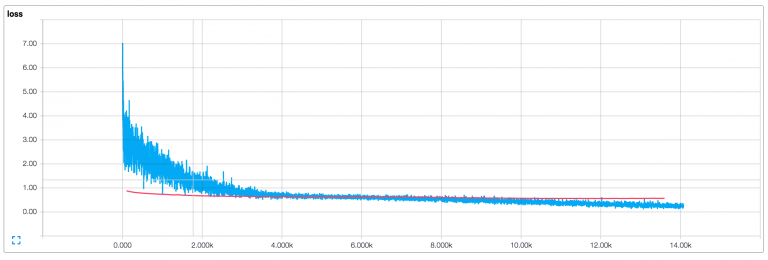
\includegraphics[width=\linewidth]{Images/cnn4.png}
	\end{center}
	\caption{Graphe qui représente les données perdues, du multiClass-SVM.}
	\label{fig:rnn}
\end{figure}
 l'état des précision qui est égale à 0,65:
\begin{figure}[H]
	\begin{center}
	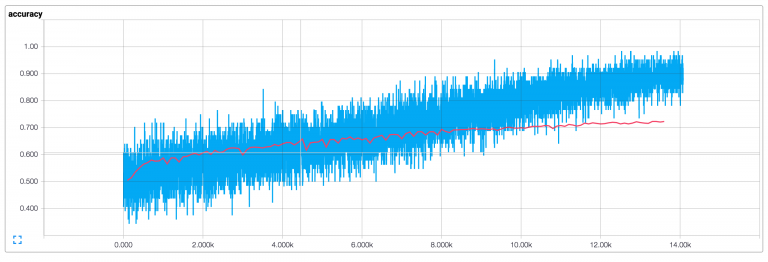
\includegraphics[width=\linewidth]{Images/cnn5.png}
	\end{center}
	\caption{Graphe qui représente la précision, du  multiClass-SVM.}
	\label{fig:rnn}
\end{figure}







\chapter{Sprint 3 : Amélioration du CNN avec word2vec}
\label{Chapitre 6} % For referencing the chapter elsewhere, use \ref{Chapter1} 

\lhead{Chapitre 6. \emph{Sprint 3 : Amélioration du CNN avec word2vec}} % This is for the header on each page - perhaps a shortened title

%----------------------------------------------------------------------------------------

\section{Spécification}
\subsection{Le Backlog du Sprint}
\begin{figure}[H]
\begin{tabular}{|p{7cm}|p{4cm}|p{4cm}|}
\hline
\textbf{Story} & \textbf{Priorité2 } & \textbf{Effort ou chargen} \\
\hline
En tant qu'utilisateur, je souhaite pouvoir visiter les différentes contenu par catégories,et de les sélectionner selon mon besoin. & \begin{center}M\end{center} & \begin{center}22\end{center}\\
\hline
\end{tabular}
  \caption{Le Backlog du Sprint 3}
  \label{fig:Backlog3}
\end{figure}
\section{Conception}
\subsection{Qu'est ce qu'un word2vec ?}
Les systèmes de traitement de l'image et du son fonctionnent avec des jeux de données riches et de grande dimension codés comme vecteurs des intensités de pixels brutes individuelles pour les données d'image, ou par exemple des coefficients de densité spectrale de puissance pour les données audio. Pour les tâches telles que la reconnaissance d'objet ou de reconnaissance vocale, nous savons que toutes les informations nécessaires à l'exécution de la tâche sont codées dans les données (car les humains peuvent effectuer ces tâches à partir des données brutes). \\[0.5cm]
Cependant, les systèmes de traitement du langage naturel traitent traditionnellement les mots comme des symboles atomiques discrets, et par conséquent, le terme 'chat' peut être représenté par Id537 'chien' Id143. Ces codages sont arbitraires et ne fournissent aucune information utile au système concernant les relations qui peuvent exister entre les symboles individuels. Cela signifie que le modèle peut tirer parti très peu de ce qu'il a appris sur les 'chats' lorsqu'il traite des données sur les 'chiens' (tels qu'ils sont à la fois des animaux, des quadrupèdes, des animaux domestiques, etc...). Le fait de représenter les mots comme des identificateurs uniques et discrets entraîne en outre un manque de données, et signifie généralement que nous aurons besoin de plus de données pour réussir la formation de modèles statistiques. L'utilisation de représentations vectorielles peut surmonter certains de ces obstacles.\\[0.5cm]
Les modèles d'espace vectoriel (VSM) représentent (incorporent) des mots dans un espace vectoriel continu où des mots sémantiquement similaires sont mappés à des points voisins ('sont imbriqués les uns près des autres'). Les VSM ont une histoire longue et riche en PNL, mais toutes les méthodes dépendent d'une manière ou d'une autre de l' hypothèse distributionnelle , qui stipule que les mots qui apparaissent dans les mêmes contextes partagent une signification sémantique. Les différentes approches qui tirent parti de ce principe peuvent être divisées en deux catégories: les méthodes fondées sur le nombre (par exemple, l' analyse sémantique latente ) et les méthodes prédictives (par exemple, les modèles de langage probabiliste neuronal ).\\[0.5cm]
Word2vec est un modèle prédictif particulièrement efficace sur le plan informatique pour l'apprentissage des plongées de mots à partir de texte brut. Il se présente sous deux formes: le modèle du sac continu de mots (CBOW) et le modèle de Skip-Gram (sections 3.1 et 3.2 de Mikolov et al.). Algorithmiquement, ces modèles sont similaires, sauf que CBOW prédit les mots cibles (par exemple 'mat') à partir des mots de contexte source ('le chat s'assoit sur le'), tandis que le skip-gram fait l'inverse et prédit les mots de contexte source de la cible mots. Cette inversion peut sembler un choix arbitraire, mais statistiquement elle a pour effet que le CBOW lisse une grande partie de l'information distributive (en traitant un contexte entier comme une observation). Pour la plupart, cela s'avère être une chose utile pour les jeux de données plus petits. Cependant, skip-gram traite chaque paire contexte-cible comme une nouvelle observation, ce qui a tendance à être meilleur lorsque nous avons des ensembles de données plus volumineux.
\subsection{Utilisation}
Ce qui m'a motivé d'utiliser le word2vect est le problème de pertes données au niveau de l'entrer du Convolutinal Neural Network du premier algorithme, et aussi le plus qui va ajouter l'approche sémantique à la precision de l'algorithme.\\
Avant l'algorithme CNN traité en input un taille de données qui est égal à 30, cette taille constante ne permettait pas de représenter la vrai valeur d'entrée, ce qui parfois déclenche une déviation sur la vrai identité de la description.\\[0.5cm]
\begin{figure}[H]
	\begin{center}
	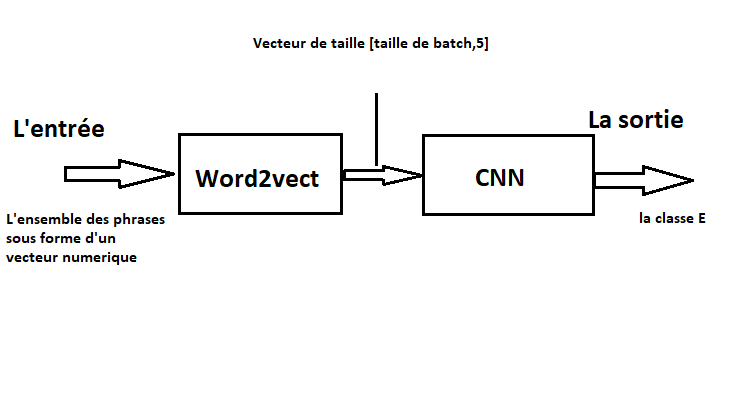
\includegraphics[width=\linewidth]{Images/w2vcnn.png}
	\end{center}
	\caption{Modélisation du modèle avec word2vect et cnn.}
	\label{fig:rnn}
\end{figure}
J'ai utilisé une taille de vecteur de word2vect égal à 5, parce que premièrement, mon corpus de données n'est pas assez grand, alors je vais économiser la mémoire, et deuxièmement pour minimiser la pertes de données au niveau de la fonction softmax.\\
La precision finale est égale à 80\%, c'est bien meilleur que les deux approches discutées au paravent.




